\documentclass[a4paper]{article}

\usepackage{amsmath,amssymb,amsfonts}
\usepackage{braket}
\usepackage{url}

\usepackage[dvipdfmx]{graphicx}

\title{Sample of GMM parameters estimation using Gibbs sampling method}
\author{Ryo Ozaki\\Ritsumeikan University\\Graduate School of Information Science and Engineering\\Emergent Systems Laboratory\\ryo.ozaki@em.ci.ritsumei.ac.jp}
\begin{document}
\maketitle
\section{Graphical model}
This section shows the graphical model of Gaussian mixture model (GMM) which were used this paper.
\begin{figure}[ht]
	\begin{center}
		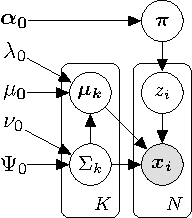
\includegraphics[width=5cm]{fig/GMM_graphical_model.pdf}
		\caption{Graphical model of GMM.}
	\end{center}
\end{figure}

The probabilistic generative process of GMM is shown below.
\begin{eqnarray}
	\lambda &=& \Set{ \alpha_0, \mu_0, \Sigma_0, \nu_0, \Psi_0 } \\
	\theta &=& \Set{ \pi, z_{1:N}, \mu_{1:K}, \Sigma_{1:K} } \\
	\nonumber \\
	\pi &\sim& {\rm Dir}(\pi | \alpha_0) \\
	\mu_k &\sim& {\rm N}(\mu_k | \mu_0, \Sigma_0) \\
	\Sigma_k &\sim& {\rm W}^{-1}(\Sigma_k | \nu_0, \Psi_0) \\
	z_i &\sim& {\rm Cat}(z_i | \pi) \\
	x_i &\sim& {\rm N}(x_i | \mu_{z_i}, \Sigma_{z_i})\\
	\nonumber \\
	k &=& 1, 2, \ldots, K\\
	i &=& 1, 2, \ldots, N
\end{eqnarray}
Here, $\lambda$ represents the set of hyperparameters, $\theta$ represents the set of parameters, ${\rm Dir}$ represents the Dirichlet distribution, ${\rm N}$ represents the normal distribution, ${\rm W}^{-1}$ represents the inverse-Wishart distribution, ${\rm Cat}$ represents the categorical distribution.

\section{Posterior distribution}
This section shows posterior distributions of the $\theta$.

\subsection{Posterior distribution of $z_i$}
The posterior distribution of $z_i$ is represented as follows.
\begin{eqnarray}
	p(z_i = k | x_i, \pi, \mu_{1:K}, \Sigma_{1:K}) &\propto& p(x_i | z_i = k, \pi, \mu_{1:K}, \Sigma_{1:K}) \nonumber \\
	&&~~~\times p(z_i = k | \pi, \mu_{1:K}, \Sigma_{1:K})\\
		&\propto& p(x_i | z_i = k, \mu_k, \Sigma_k) p(z_i = k | \pi)\\
	&=& {\rm N}(x_i | \mu_k, \Sigma_k) {\rm Cat(z_i = k | \pi)}\\
	&=& {\rm Cat}(z_i = k | \hat{\pi})\\
	\nonumber \\
	\hat{\pi}^{-}_{k} &=& {\rm N}(x_i | \mu_k, \Sigma_k) \times \pi_k \\
	\hat{\pi}_k &=& \frac{\hat{\pi}^{-}_k}{\sum_{l = 1}^{K}{\hat{\pi}^{-}_l}}
\end{eqnarray}

\subsection{Posterior distribution of $\pi$}
The posterior distribution of $\pi$ is represented as follows.
\begin{eqnarray}
	p(\pi | \alpha_0, z_{1:N}) &\propto& p(z_{1:N} | \pi, \alpha_0) p(\pi | \alpha_0)\\
	&\propto& p(z_{1:N} | \pi) p(\pi | \alpha_0)\\
	&=& \prod_{i=1}^{N}{\left\{ p(z_i | \pi) \right\} } p(\pi | \alpha_0)\\
	&=& \prod_{i=1}^{N}{\left\{ {\rm Cat}(z_i | \pi) \right\} } {\rm Dir}(\pi | \alpha_0)\\
	&=& {\rm Mult}(m | \pi) {\rm Dir}(\pi | \alpha_0)\\
	&=& {\rm Dir}(\pi | \hat{\alpha})\\
	\nonumber \\
	m_k &=& \sum_{i=1}^{N}{\delta(z_i = k)}\\
	\delta(\text{CONDITION}) &=&
	\left\{
	\begin{array}{ll}
		0 & (\text{CONDITION is false})\\
		1 & (\text{CONDITION is true})
	\end{array}
	\right.\\
	\hat{\alpha} &=& m + \alpha_0
\end{eqnarray}
Here, ${\rm Mult}$ represents multinomial distribution.

\subsection{Posterior distribution of $\Sigma_k$}
The posterior distribution of $\Sigma_k$ is represented as follows.
\begin{eqnarray}
	p(\Sigma_k | \nu_0, \Psi_0, x_{1:N}, z_{1:N}, \mu_k) &=& p(\Sigma_k | \nu_0, \Psi_0, x^{k}_{1:M}, \mu_k)\\
	&\propto& p(x^{k}_{1:M} | \nu_0, \Psi_0, \mu_k, \Sigma_k) p(\Sigma_k | \nu_0, \Psi_0, \mu_k)\\
	&\propto& p(x^{k}_{1:M} | \mu_k, \Sigma_k) p(\Sigma_k | \nu_0, \Psi_0)\\
	&=& \prod_{j=1}^{M}{\left\{ p(x^{k}_{j} | \mu_k, \Sigma_k) \right\}} p(\Sigma_k | \nu_0, \Psi_0)\\
	&=& \prod_{j=1}^{M}{\left\{ {\rm N}(x^{k}_{j} | \mu_k, \Sigma_k) \right\}} {\rm W}^{-1}(\Sigma_k | \nu_0, \Psi_0)\\
	&=& {\rm W}^{-1}(\Sigma_k | \hat{\nu}, \hat{\Psi})\\
	\nonumber \\
	x^{k}_{1:M} &=& \Set{ x_i | z_i = k, i=1, \ldots, N }\\
	m_k &=& \sum_{i=1}^{N}{\delta(z_i = k)}\\
	\hat{\nu} &=& m_k + \nu_0\\
	\hat{\Psi} &=& \sum_{j=1}^{M}{\left\{ \left(x_j - \mu_k \right) \cdot \left( x_j - \mu_k \right)^T \right\}} + \Psi_0
\end{eqnarray}

\subsection{Posterior distribution of $\mu_k$}
The posterior distribution of $\mu_k$ is represented as follows.
\begin{eqnarray}
	p(\mu_k | \mu_0, \Sigma_0, x_{1:N}, z_{1:N}, \Sigma_k) &=& p(\mu_k | \mu_0, \Sigma_0, x^{k}_{1:M}, \Sigma_k)\\
	&\propto& p(x^{k}_{1:M} | \mu_0, \Sigma_0, \mu_k, \Sigma_k) p(\mu_k | \mu_0, \Sigma_0, \Sigma_k)\\
	&\propto& p(x^{k}_{1:M} | \mu_k, \Sigma_k) p(\mu_k | \mu_0, \Sigma_0)\\
	x^{k}_{1:M} &=& \left\{ x_i | z_i = k, i=1, \ldots, N \right\}\\
	&=& \prod_{j=1}^{M}{\left\{ p(x^{k}_{j} | \mu_k, \Sigma_k) \right\}} p(\mu_k | \mu_0, \Sigma_0)\\
	&=& \prod_{j=1}^{M}{\left\{ {\rm N}(x^{k}_{j} | \mu_k, \Sigma_k) \right\}} {\rm N}(\mu_k | \mu_0, \Sigma_0)\\
	&=& {\rm N}(\mu_k | \hat{\mu}, \hat{\Sigma})\\
	\nonumber \\
	x^{k}_{1:M} &=& \Set{ x_i | z_i = k, i=1, \ldots, N }\\
	m_k &=& \sum_{i=1}^{N}{\delta(z_i = k)}\\
	\hat{\Sigma} &=& \left( m_k \Sigma^{-1}_k + \Sigma^{-1}_0 \right)^{-1}\\
	\hat{\mu} &=& \hat{\Sigma} \cdot \left\{ \Sigma^{-1}_k \cdot \sum_{j=1}^{M}{\left( x^k_j \right) + \Sigma^{-1}_0 \cdot \mu_0} \right\}
\end{eqnarray}

\section{Experiments}
This section shows results of experiments.

\subsection{Truth parameters}
Parameters which were used in this experiments represented follows.
\begin{eqnarray}
	\pi^* &=& \left[ \begin{array}{ccc}
		0.7 & 0.2 & 0.1
	\end{array}
	\right]\\
	\mu^*_{1:3} &=& 
	\left[\begin{array}{c}
		3.0\\
		0.0
	\end{array}\right]
	, 
	\left[\begin{array}{c}
		-3.0\\
		0.0
	\end{array}\right]
	, 
	\left[\begin{array}{c}
		0.0\\
		5.0
	\end{array}\right]\\
	\Sigma^*_{1:3} &=& 
	\left[\begin{array}{cc}
		1.0 & 0.0\\
		0.0 & 1.0
	\end{array}\right]
	, 
	\left[\begin{array}{cc}
		1.0 & 0.0\\
		0.0 & 1.0
	\end{array}\right]
	, \left[\begin{array}{cc}
		1.0 & 0.0\\
		0.0 & 1.0
	\end{array}\right]
\end{eqnarray}

\subsection{Hyperparameters}
Hyperparameters which were used in this experiments represented follows.
\begin{eqnarray}
	\alpha_0 &=& \left[\begin{array}{ccc} 1.0 & 1.0 & 1.0 \end{array}\right]\\
	\mu_0 &=& \left[\begin{array}{c}
		0.0\\
		0.0
	\end{array}\right]\\
	\Sigma_0 &=& \left[\begin{array}{cc}
		1.0 & 0.0\\
		0.0 & 1.0
	\end{array}\right]\\
	\nu_0 &=& 2.0\\
	\Psi_0 &=& \left[\begin{array}{cc}
		1.0 & 0.0\\
		0.0 & 1.0
	\end{array}\right]
\end{eqnarray}

\subsection{Experiment 1}
This section shows a clustering result of the dataset which has 300 observations.
Figure \ref{fig:ex1_truth} shows the dataset which are used in this experiment.
In addition, we set $K = 4$ which is a number of clusters.
We did Gibbs sampling 150 steps.
\begin{figure}[h]
	\begin{center}
		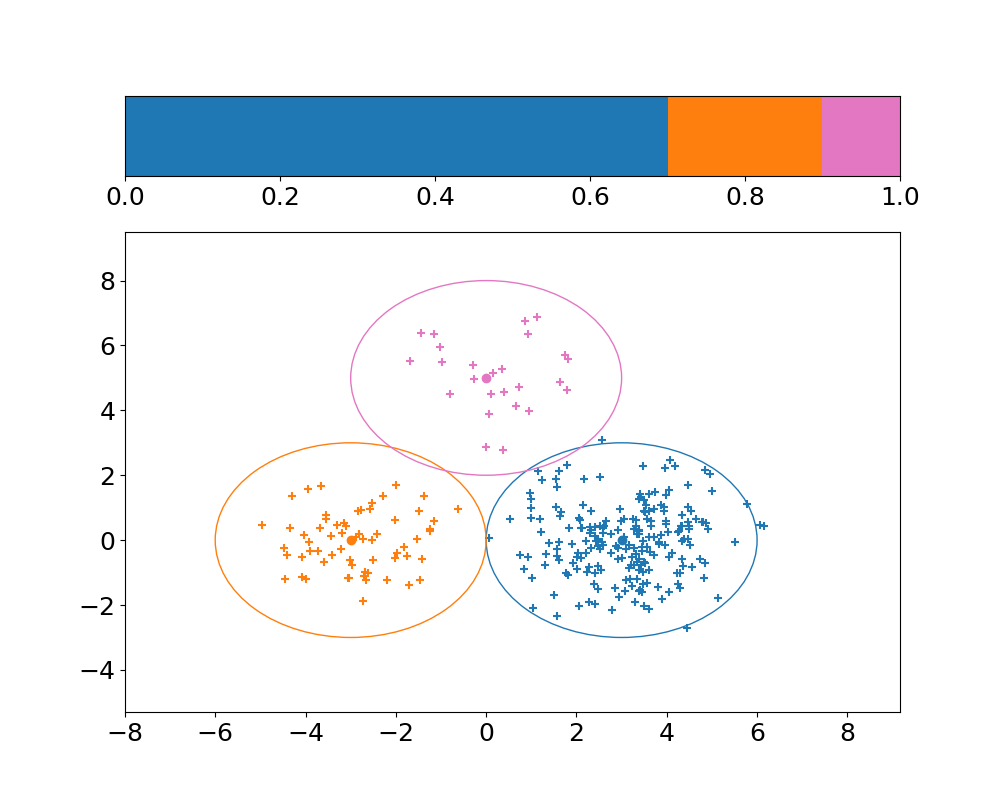
\includegraphics[width=11cm]{fig/ex1/truth.png}
		\caption{Truth data (300 points)}
		\label{fig:ex1_truth}
	\end{center}
\end{figure}

Figure \ref{fig:ex1_result} shows a result at 150-th step in Gibbs sampling.
In addition, you can see the process of Gibbs sampling at the file named ``GMM\_Gibbs\_result1.gif'' which in this directory.
Also, you can see the stochastic behavior of Gibbs sampling.
\begin{figure}[h]
	\begin{center}
		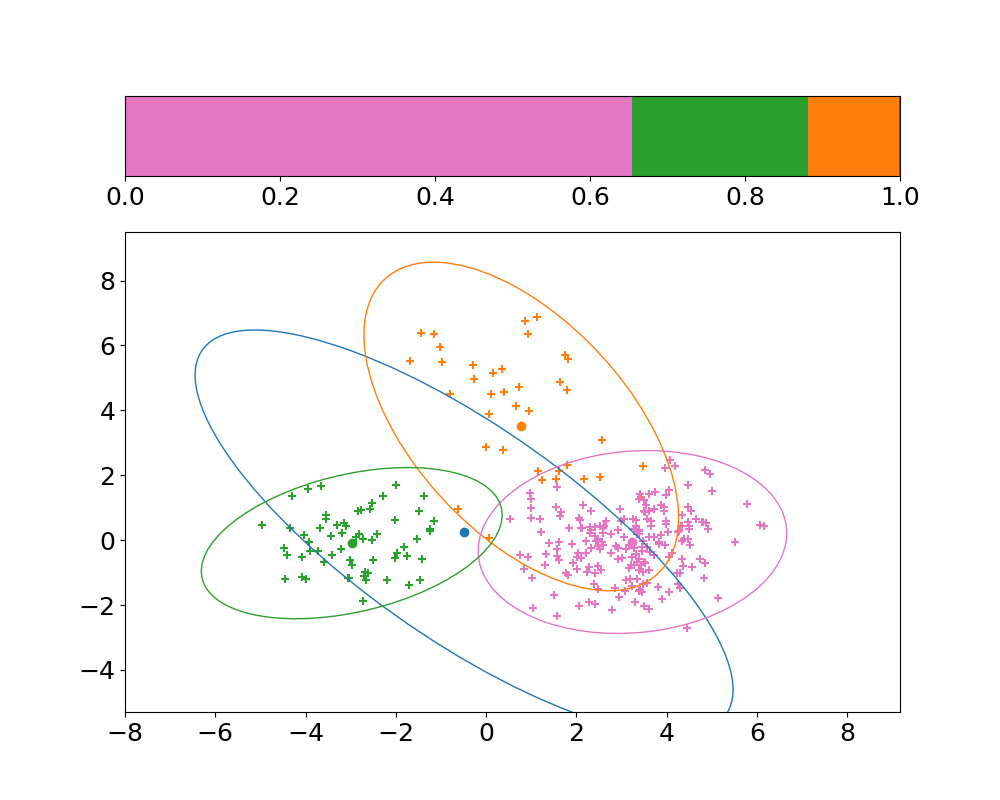
\includegraphics[width=11cm]{fig/ex1/final.png}
		\caption{Result at 150-th step in Gibbs sampling}
		\label{fig:ex1_result}
	\end{center}
\end{figure}

\subsection{Experiment 2}
This section shows a clustering result of the dataset which has 3000 observations.
Figure \ref{fig:ex2_truth} shows the dataset which are used in this experiment.
Other conditions are same as is experiment 1.
\begin{figure}[h]
	\begin{center}
		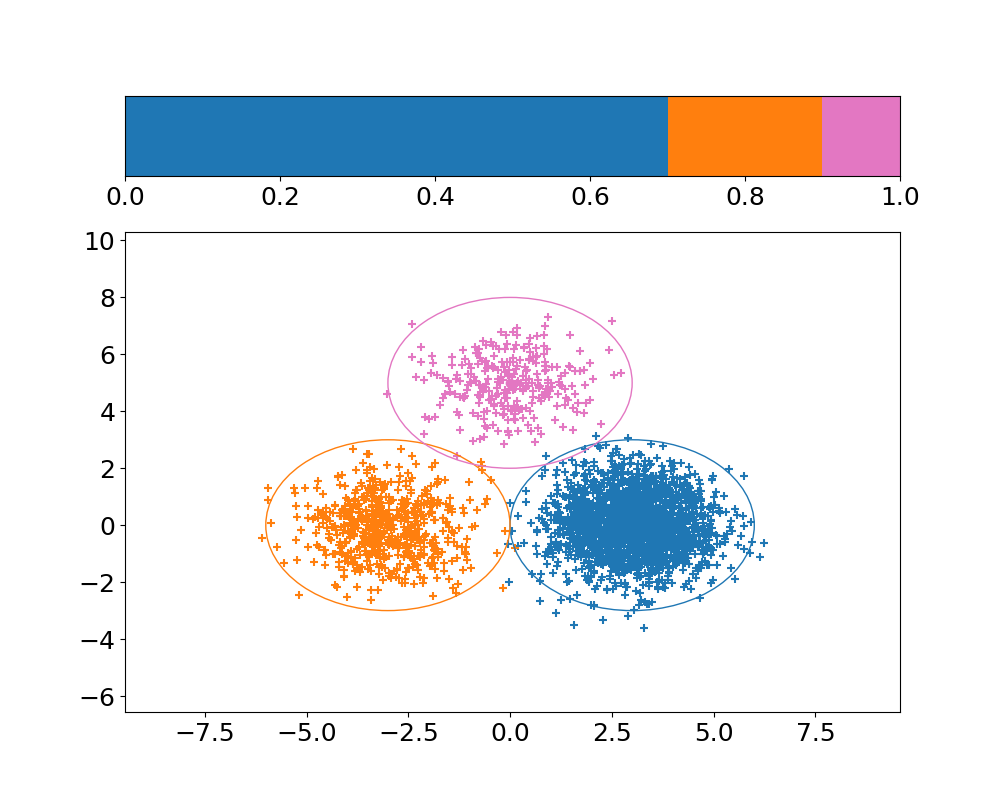
\includegraphics[width=11cm]{fig/ex2/truth.png}
		\caption{Truth data (3000 points)}
		\label{fig:ex2_truth}
	\end{center}
\end{figure}

Figure \ref{fig:ex2_result} shows a result at 150-th step in Gibbs sampling.
In addition, you can see the process of Gibbs sampling at the file named ``GMM\_Gibbs\_result2.gif'' which in this directory.
\begin{figure}[h]
	\begin{center}
		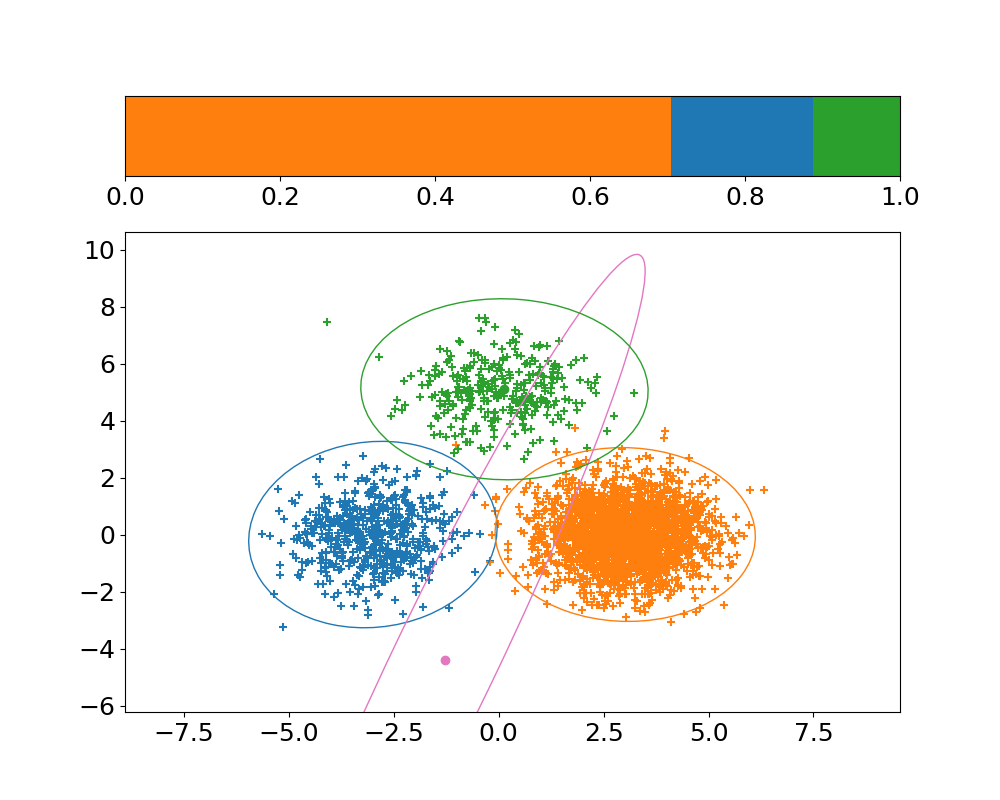
\includegraphics[width=11cm]{fig/ex2/final.png}
		\caption{Result at 150-th step in Gibbs sampling}
		\label{fig:ex2_result}
	\end{center}
\end{figure}

\newpage
\section{Summary}
This paper derived the posterior distributions of parameters $\theta$.
In addition, we estimated the parameters of synthesis dataset which has 300 and 3000 observations.
Also, we showed the stochastic behavior of Gibbs sampling into ``GMM\_Gibbs\_result1.gif'' and ``GMM\_Gibbs\_result2.gif.''

You can the same experiment on your computer using this GitHub repository.
If you want to do, please run following commands.
\begin{enumerate}
	\item \verb|git clone https://github.com/RyoOzaki/GibbsSampling|\\
		Clone this repository to your computer.
	\item \verb|cd GibbsSampling/GMM|\\
		Change directory to ``GMM'' in ``GibbsSampling''.
	\item \verb|python GMM_Gibbs.py|\\
		Run Gibbs sampling. You can get result in ``tmp'' directory.
	\item \verb|sh make_gif.sh|\\
		Convert images in ``tmp'' directory to ``result.gif.''
\end{enumerate}


\end{document}
